\section{Programming}
\label{sec:program}
\begin{frame}<beamer>
    \frametitle{Outline}
    \tableofcontents[currentsection]
\end{frame}

\begin{frame}
	\frametitle{Why programming? (1)}
	\begin{figure}
	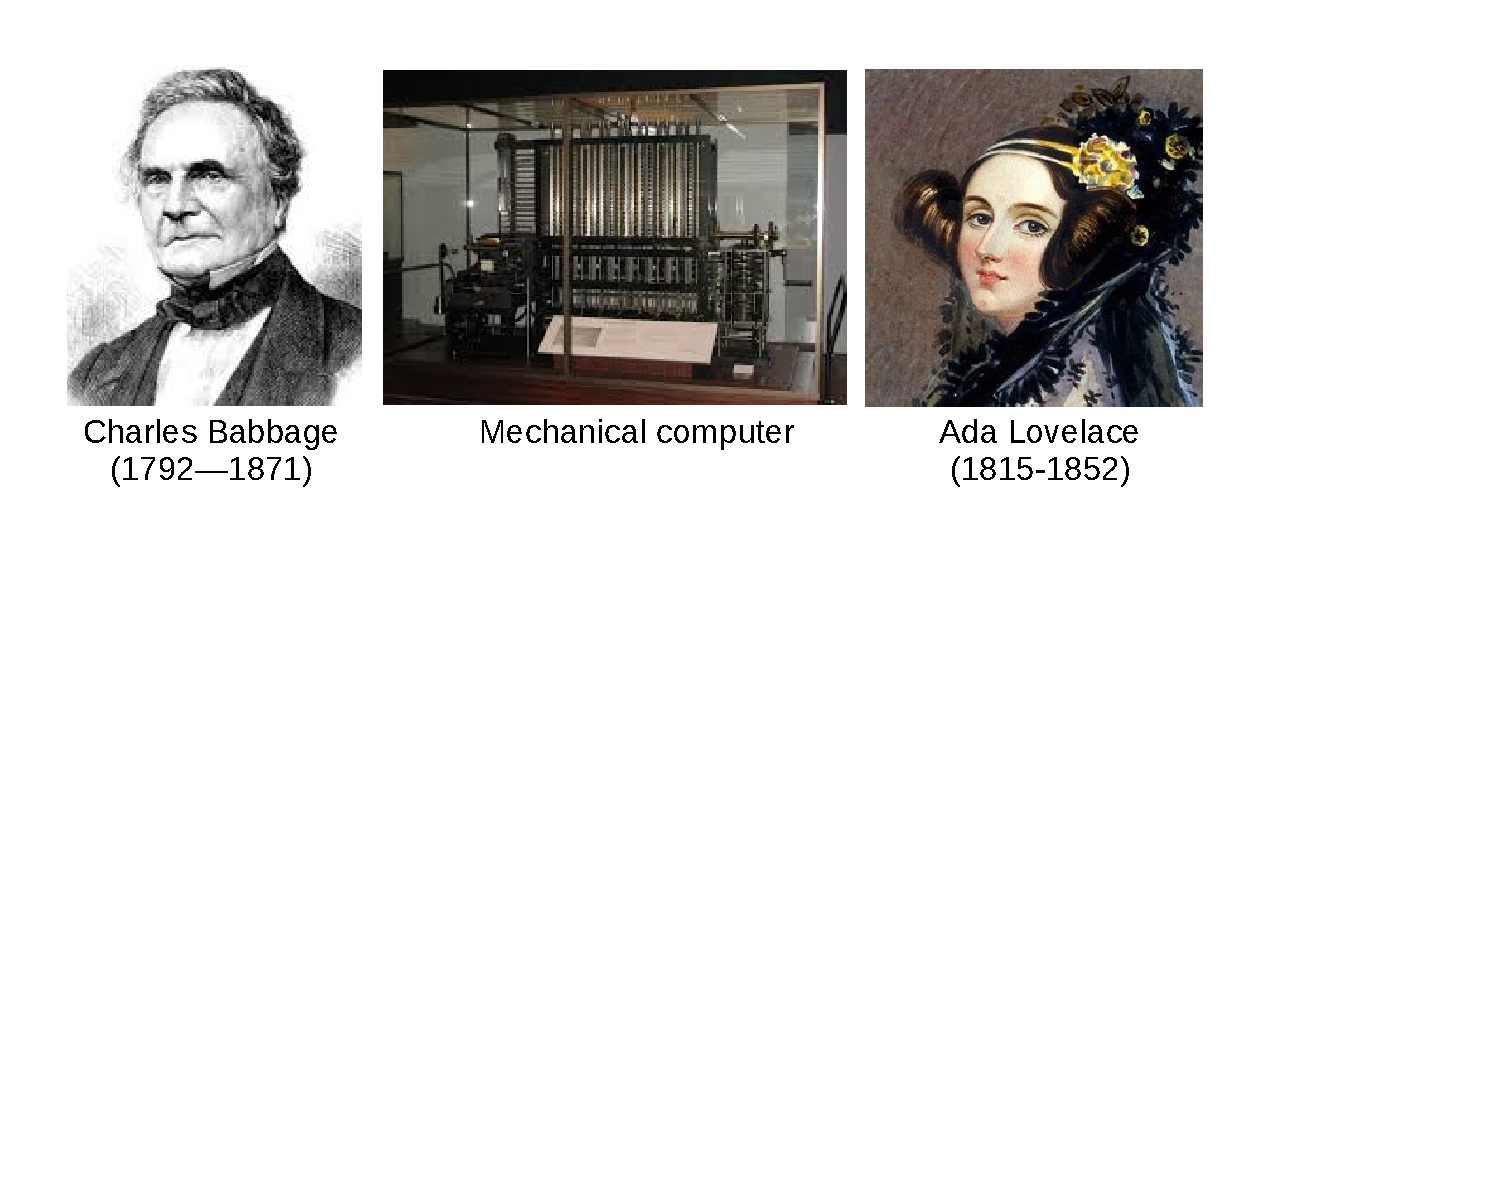
\includegraphics[width=0.85\linewidth]{figs/ada.pdf}
\end{figure}
\begin{itemize}
	\item {Ada is the first programmer}
	\item {A language is named after her to memorize her contribution}
\end{itemize}
\end{frame}

\begin{frame}
	\frametitle{Why programming? (2)}
	\begin{figure}
	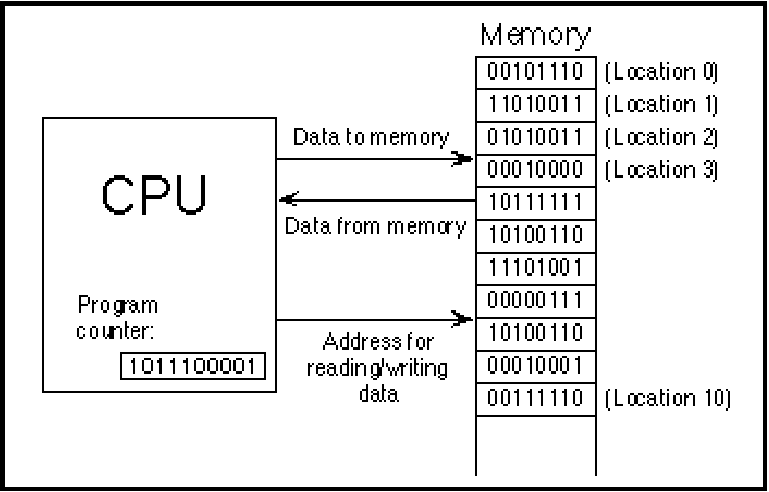
\includegraphics[width=0.65\linewidth]{figs/workflow.pdf}
\end{figure}
\begin{itemize}
	\item {Instructions and data fetch from memory to CPU for processing}
	\item {The results are returned back to memory}
\end{itemize}
\end{frame}

\begin{frame}
	\frametitle{Why High Level Programming Language? (1)}
\begin{figure}
	
\includegraphics[width=0.75\linewidth]{figs/talk2pc.pdf}
\end{figure}
\begin{itemize}
	\item {Natural language is the media that we communicate with each other}
	\item {Computer language is the media that we communicate with computer}
	\item {We should use the language that computer could understand}
	\item {At least, we need an \textcolor{red}{interpreter/translator}}
\end{itemize}
\end{frame}

\begin{frame}
	\frametitle{Why High Level Programming Language? (2)}
	\begin{figure}
	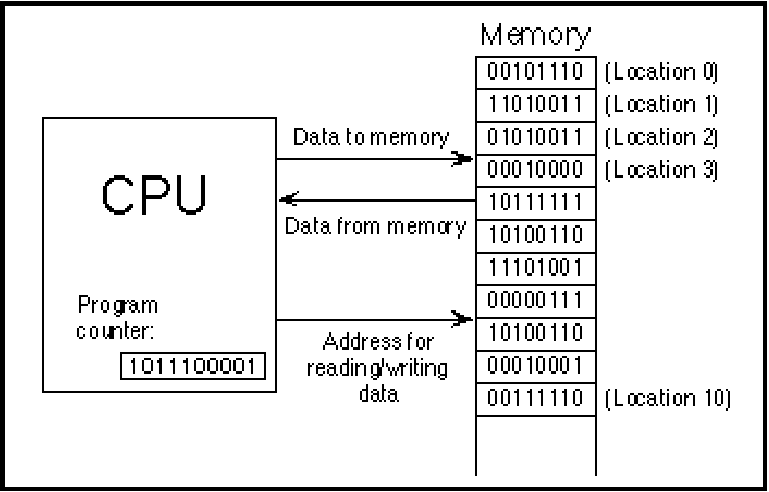
\includegraphics[width=0.65\linewidth]{figs/workflow.pdf}
\end{figure}
\begin{itemize}
	\item {Instructions are binary codes}
	\item {Machine only accepts/understands binary codes}
\end{itemize}
\end{frame}

\begin{frame}
	\frametitle{Why Programming Language? (3)}
\begin{columns}
\begin{column}{0.45\linewidth}
\begin{enumerate}
	\item {010101 0000 0011}
	\item {010101 0001 0101}
	\item {101010 0000 0001}
	\item {010101 0000 1011}
\end{enumerate}
\end{column}
\end{columns}
\end{frame}

\begin{frame}
	\frametitle{Why Programming Language? (4)}
\begin{columns}
\begin{column}{0.45\linewidth}
\begin{enumerate}
	\item {010101 0000 0011}
	\item {010101 0001 0101}
	\item {101010 0000 0001}
	\item {010101 0000 1011}
\end{enumerate}
\end{column}
\begin{column}{0.45\linewidth}
\vspace{-0.1in}
\begin{enumerate}
	\item {MOV D1 0011}
	\item {MOV D2 0101}
	\item {ADD D1 D2}
	\item {MOV D1 A1}
\end{enumerate}
\end{column}
\end{columns}
\vspace{0.2in}
\begin{itemize}
	\item {For the convenience of operation, binary instructions are denoted with readable symbols}
\end{itemize}

\end{frame}

\begin{frame}
	\frametitle{Why Programming Language? (5)}
\begin{columns}
\begin{column}{0.4\linewidth}
\begin{itemize}
	\item {Machine code}
\end{itemize}
\begin{enumerate}
	\item {010101 0000 0011}
	\item {010101 0001 0101}
	\item {101010 0000 0001}
	\item {010101 0000 1011}
\end{enumerate}
\end{column}
\begin{column}{0.3\linewidth}
\vspace{-0.1in}
\begin{itemize}
	\item {Assembly}
\end{itemize}
\begin{enumerate}
	\item {MOV D1 0011}
	\item {MOV D2 0101}
	\item {ADD D1 D2}
	\item {MOV D1 A1}
\end{enumerate}
\end{column}
\begin{column}{0.25\linewidth}
\vspace{-0.1in}
\begin{itemize}
	\item {High level language}
\end{itemize}
\begin{enumerate}
	\item {a=3+5;}
\end{enumerate}
\end{column}
\end{columns}
\end{frame}

\begin{frame}
	\frametitle{Why Programming Language? (6)}
\begin{figure}
	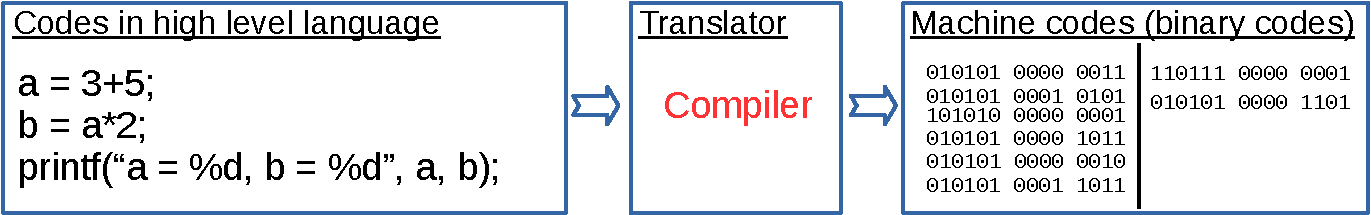
\includegraphics[width=0.95\linewidth]{figs/compil.pdf}
\end{figure}
\begin{itemize}
	\item {We write a \textcolor{red}{text} file in specified format (grammar)}
	\item {These are instructions that we basically understand}
	\item {The \textcolor{red}{translator} converts the text instructions into machine codes}
	\item {Machine then runs these binary codes one by one}
	\item {Different \textcolor{red}{translator}s lead to different programming languages}
	\item {Which also regulate different grammars}
	\item {C is such kind of high level language}
\end{itemize}
\end{frame}

\begin{frame}
	\frametitle{The life-time of a computer program}
\begin{figure}
	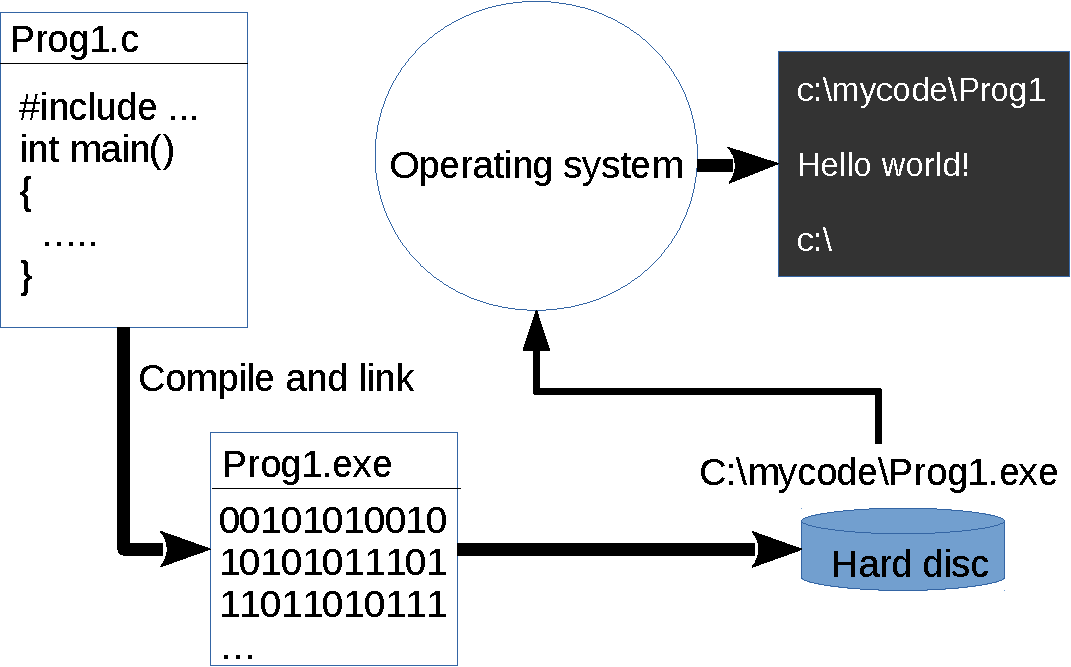
\includegraphics[width=0.95\linewidth]{figs/life-tm.pdf}
\end{figure}
\end{frame}